\documentclass[a4paper,11pt]{article}
\usepackage{amssymb, enumitem}

\parindent 0cm
\usepackage{amssymb,amsmath,amsthm,latexsym,epsfig,euscript,multicol}
\usepackage[utf8x]{inputenc}
\usepackage{listings,xcolor,bm}


\definecolor{mygreen}{rgb}{0,0.6,0}
\definecolor{mygray}{rgb}{0.5,0.5,0.5}
\definecolor{mymauve}{rgb}{0.58,0,0.82}
\lstset{
  backgroundcolor=\color{white},   % choose the background color; you must add
  basicstyle=\small\ttfamily,      % the size of the fonts that are used for the code
  breakatwhitespace=false,         % sets if automatic breaks should only happen at whitespace
  breaklines=true,                 % sets automatic line breaking
  captionpos=b,                    % sets the caption-position to bottom
  commentstyle=\color{mygreen},    % comment style
  deletekeywords={...},            % if you want to delete keywords from the given language
  escapeinside={\%*}{*)},          % if you want to add LaTeX within your code
  extendedchars=true,              % lets you use non-ASCII characters; for 8-bits encodings only, does not work with UTF-8
  firstnumber=1,                % start line enumeration with line 1000
  frame=single,	                   % adds a frame around the code
  keepspaces=true,                 % keeps spaces in text, useful for keeping indentation of code (possibly needs columns=flexible)
  keywordstyle=\color{blue},       % keyword style
  language=Python,                 % the language of the code
  morekeywords={*,...},            % if you want to add more keywords to the set
  numbers=left,                    % where to put the line-numbers; possible values are (none, left, right)
  numbersep=5pt,                   % how far the line-numbers are from the code
  numberstyle=\tiny\color{mygray}, % the style that is used for the line-numbers
  rulecolor=\color{black},         % if not set, the frame-color may be changed on line-breaks within not-black text (e.g. comments (green here))
  showspaces=false,                % show spaces everywhere adding particular underscores; it overrides 'showstringspaces'
  showstringspaces=false,          % underline spaces within strings only
  showtabs=false,                  % show tabs within strings adding particular underscores
  stepnumber=5,                    % the step between two line-numbers. If it's 1, each line will be numbered
  stringstyle=\color{mymauve},     % string literal style
  tabsize=4,	                   % sets default tabsize to 2 spaces
  title=\lstname,                  % show the filename of files included with \lstinputlisting; also try caption instead of title
  numbers=none
}
% Caracteres especiales
\def\A{\mathbb{A}}
\def\C{\mathbb{C}}
\def \N{\mathbb{N}}
\def \P{\mathbb{P}}
\def \Q{\mathbb{Q}}
\def \R{\mathbb{R}}
\def \Z{\mathbb{Z}}
\def \sen{\textrm{sen}}

\def\Np{$\N$}
\def\Zp{$\Z$}
\def\Qp{$\Q$}
\def\Rp{$\R$}
\def\Cp{$\C$}

\def\bb{\bm{b}}
\def\bu{\bm{u}}
\def\bv{\bm{v}}
\def\bx{\bm{x}}
\def\bA{\bm{A}}
\def\bB{\bm{B}}
\def\bD{\bm{D}}
\def\bE{\bm{E}}
\def\bM{\bm{M}}
\def\bT{\bm{T}}


\def\K{\textrm{K}}
\def\V{\textrm{V}}
\def\S{\textrm{S}}

\def\degres{$^\circ$}

\newcount\todno
\def\no{\global\advance\todno by 1 \the\todno}

\topmargin-2cm \vsize 29.5cm \hsize 21cm
\setlength{\textwidth}{16.75cm}\setlength{\textheight}{23.5cm}
\setlength{\oddsidemargin}{0.0cm}
\setlength{\evensidemargin}{0.0cm}


\theoremstyle{definition}
\newtheorem{ejer}{Ejercicio}
\newcommand{\bej}{\begin{ejer}}
\newcommand{\fej}{\end{ejer}}

\begin{document}

\centerline{{\small Universidad de Buenos Aires - Facultad de Ciencias Exactas y Naturales - Ciencias de Datos}}

\vskip 0.2cm

\hrule

\vskip 0.2cm

 \centerline{{\bf\Large{\sc Laboratorio de Datos}}}

 \vskip 0.2cm

 \centerline{\ttfamily Primer Cuatrimestre 2024}

\vskip 0.2cm

 \hrule

 \bigskip
 \centerline{\bf Práctica N$^\circ$ 2: Estad\'istica descriptiva}
 \bigskip


\textbf{\large Estructuras de datos en Pandas}

\vspace{0.2cm}

\textbf{Series.} Las series de Pandas son vectores similares a los arrays de NumPy, que podemos indexar usando etiquetas.

\begin{enumerate}
\item Crear la siguiente Series, observar qué devuelve \lstinline{array} e \lstinline{index} e interpretar.

\begin{lstlisting}
import pandas as pd
obj = pd.Series([7,4,-5,3])
display(obj)
display(obj.array)
display(obj.index)  # Por default, los indices van de 0 a N-1.
\end{lstlisting}

\item Podemos asignar etiquetas (o \'indices) a cada valor de la serie.
\begin{lstlisting}
obj2 = pd.Series([np.pi,0,-2,1.41], index = ["d", "b", "c", "a"])
display(obj2)
display(obj2.array)
display(obj2.index)
\end{lstlisting}

\item Al igual que con arrays de Numpy podemos acceder a los elementos por su posici\'on, o podemos usar las etiquetas. Ejecutar los siguientes comandos.
\begin{lstlisting}
obj2["a"]
obj2[3]
obj2[1:3]

obj3 = obj2[["a","b"]]
obj3
obj3.index

obj2[obj2>1]
\end{lstlisting}

\item Las operaciones que pueden aplicarse a numpy arrays pueden aplicarse tambi\'en a series de Pandas, conservando los \'indices.
\begin{lstlisting}
np.exp(obj2)
obj2 * 3
\end{lstlisting}

\item \textbf{M\'etodos de series.} Ejecutar los siguientes comandos e interpretar qu\'e hace cada uno.
\begin{lstlisting}
series1 = pd.Series(["a", "b", "c", "b", "a", "c", "c", "x"])
series1.isin(["b", "c"])
series1.value_counts()
\end{lstlisting}

\end{enumerate}

\textbf{DataFrames.} Un DataFrame es una representaci\'on de los datos en formato de tabla donde las columnas son vectores del mismo tama\~no. Como cada columna es un vector, cada columna puede contener datos de un \'unico tipo. Se pueden pensar como variables. Cada variable corresponde a una serie de Pandas, y todas las series de un mismo DataFrame est\'an indexadas por los mismos \'indices.

\begin{enumerate}[resume]
\item Una forma de crear un DataFrame es utilizando un ``diccionario''. Todas las variables del diccionario deben ser vectores o listas de la misma longitud. Ejecutar el siguiente c\'odigo.

\begin{lstlisting}
data = {"nombre": ["Rodrigo", "Sergio", "Cristina", "Diana"], "altura": np.array([178, 172, 175, 168]), "peso": np.array([81.2, 76.1, 68.5, 64.0])}
display(data)

pacientes = pd.DataFrame(data).set_index("nombre")
display(pacientes)
\end{lstlisting}

\item ?`Cu\'al es la clase del objeto \lstinline{pacientes}? ?`Cu\'al es la clase de cada uno de los vectores columna? (para saber la clase de un objeto, utilizar el comando \lstinline{type}, para saber el tipo de datos de un array de numpy, utilizar \lstinline{np.dtype})

\item Guardar en una variable nueva el vector columna \lstinline{altura}. Pueden utilizar \lstinline{pacientes["altura"]} o \lstinline{pacientes.altura} (la primera opci\'on es preferible, la segunda puede dar error si el nombre coincide con alguna funci\'on ya existente).

\item A diferencia de las matrices en Numpy, un DataFrame de Pandas es un conjunto de columnas, no de filas. Pensar cu\'al de los dos comandos ser\'a correcto antes de ejecutarlos.
\begin{lstlisting}
pacientes["Rodrigo"].altura
pacientes["altura"].Rodrigo
\end{lstlisting}


\item \textbf{Gapminder.} A modo de ejemplo, vamos a explorar el DataFrame \lstinline{gapminder} que contiene datos poblacionales y de desarrollo humano de distintos pa\'ises a lo largo del tiempo.

    Cargar la biblioteca \lstinline{gapminder} utilizando
\begin{lstlisting}
from gapminder import gapminder
\end{lstlisting}
Si da error es posible que no est\'e instalado. En tal caso ejecuten primero
\begin{lstlisting}
pip install gapminder
\end{lstlisting}
Esto crea un nuevo objeto \lstinline{gapminder}. Pueden ver el contenido con el comando con algunos de estos comandos: \lstinline{display(gapminder)}, \lstinline{gapminder.info()}, \lstinline{gapminder.head()}, \lstinline{gapminder.tail()}.

\item ?`De qu\'e clase es el objeto \lstinline{gapminder}? ?`Qu\'e variables tiene el DataFrame \lstinline{gapminder} y de qu\'e clase son? ?`Qu\'e \'indices usa?

\item Explorar el tama\~no del DataFrame \lstinline{gapminder} usando la funci\'on \lstinline{shape}.

\item ?`De cu\'antos pa\'ises hay datos? Ayuda: averiguar qu\'e hacen los m\'etodos \lstinline{unique()} y \lstinline{nunique()} aplicados a series.


%\item ?`Cu\'ales son las variables? Usar el comando \lstinline{gapminder.columns.values}.

\item Extraer la informaci\'on de Argentina, Uruguay y Chile y guardarla en un nuevo DataFrame \lstinline{gm_sur}. Sugerencia: recordar el m\'etodo \lstinline{isin()}.

?`Cu\'antas filas tiene? ?`Cu\'al es el primer y el \'ultimo a\~no para el cu\'al existen datos de Argentina en \lstinline{gapminder}?

\item ?`C\'omo est\'a indexado el DataFrame \lstinline{gm_sur}? Para acceder a una fila de un DataFrame, podemos usar los m\'etodos \lstinline{loc[]} y \lstinline{iloc[]}. ?`C\'omo se usan? ?`Cu\'al es la diferencia entre los dos comandos?

%\item ?`Qu\'e resulta de hacer gm.sur[,"pop"]? ?`Qu\'e resulta de hacer gm.sur[,-(1:3)]?

\end{enumerate}

\textbf{\large Archivos de datos}

\begin{enumerate}[resume]
\item La biblioteca \lstinline{Pandas} nos permite tambi\'en trabajar con archivos de datos.

\begin{enumerate}
\item Leer el archivo \lstinline{casos_coronavirus.csv}.
\item Graficar la curva de casos por d\'ia.
\item Graficar la curva de casos acumulados (utilizar la funci\'on \lstinline{cum_sum} para calcularlos.
\item Definir $y$ como el logaritmo de la cantidad de casos acumulados y graficar $y$ en funci\'on de la cantidad de d\'ias transcurridos.
\end{enumerate}
Utilicen el siguiente c\'odigo para leer el archivo y graficar.

\begin{lstlisting}
df = pd.read_csv("casos_coronavirus.csv")   # dataFrame
df

df["confirmados_Nuevos"].plot()
\end{lstlisting}

\end{enumerate}

\textbf{\large Estad\'istica descriptiva}
\begin{enumerate}[resume]

\item Dar tres ejemplos de variables categ\'oricas y num\'ericas.

\item En el DataFrame \lstinline{gapminder}, una de las variables es el producto bruto per capita de los pa\'ises (gdpPercap). ?`Es una variable categ\'orica (nominal u ordinal) o num\'erica (discreta o continua)?

\item Supongamos que definimos una nueva variable que puede tomar los siguientes valores:
\[
\text{nivelGDP} = \begin{cases}
0, & \text{si \lstinline{gdpPercap}} < 1600. \\
1, & \text{si $1600 \le $ \lstinline{gdpPercap} $< 6600$}. \\
2, & \text{en otro caso.} \\
\end{cases}
\]
?`La nueva variable
 es categ\'orica (nominal u ordinal) o num\'erica (discreta o continua)? ?`Cambia la respuesta si la variable
 toma valores ``bajo'', ``medio'' y ``alto'' en lugar de 0, 1, 2?

\item Filtrar el DataFrame de \lstinline{gapminder} para el a\~no 2007. Luego, para ese a\~no, calcular la cantidad de pa\'ises en cada continente. Explorar la función \lstinline{groupBy()} y los métodos \lstinline{size()} y \lstinline{nunique()} de un DataFrame agrupado.

\item Con el mismo filtro que el ejercicio anterior (es decir, s\'olo para el a\~no 2007), crear una variable $gdpAlto$
 que valga 1 si \lstinline{gdpPercap} es mayor que 2000 d\'olares y 0 si no lo es. Luego crear una tabla de 2 filas y 5 columnas que calcule la cantidad de pa\'ises donde $gdpAlto = 0$ o $gdpAlto = 1$  en cada continente. 
 
 Ayuda 1: para convertir un array de variables booleanas a 0/1 pueden usar \lstinline{.astype(int)} (o en este ejercicio pueden usar una variable booleana en vez de 0/1).
 
 Ayuda 2: si tenemos informaci\'on agrupada por 2 columnas, podemos convertirla a una tabla con la funci\'on \lstinline{unstack()}.

%\item Convertir el vector colores a factor y comprobar que funcion\'o usando la funci\'on \lstinline{class()}. Verificar las categor\'ias creadas usando la funci\'on \lstinline{levels()}.
%\begin{lstlisting}
%colores <- c('blue', 'red', 'green', 'red', 'black', 'yellow','blue','blue')
%\end{lstlisting}

\item En el gr\'afico vemos 11 puntos. Consideramos la media y mediana de la coordenada $x$ de esos puntos y graficamos dos rectas verticales $x = $ media y $x = $ mediana. ?`Cu\'al recta corresponde a la media y cu\'al a la mediana?

\begin{center}
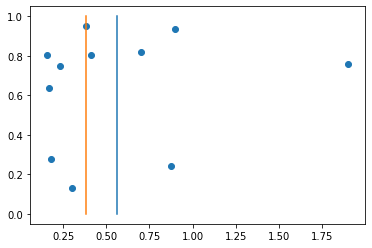
\includegraphics[scale=0.6]{practica2-img-media_mediana_1.png}
\end{center}

\item Repetimos el mismo procedimiento con otros 30 puntos. Graficamos una l\'inea azul para la media y una l\'inea naranja para la mediana. Uno de los dos gr\'aficos es correcto, ?`cu\'al?

\begin{center}
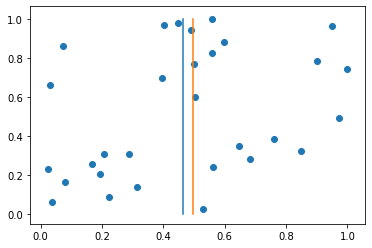
\includegraphics[scale=0.5]{practica2-img-media_mediana_2.png}
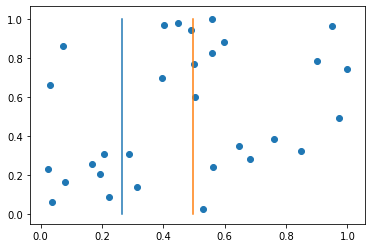
\includegraphics[scale=0.5]{practica2-img-media_mediana_3.png}
\end{center}


\item Definir funciones que calculen la media y mediana de un vector de valores num\'ericos.

\item Probar las funciones definidas con las variables num\'ericas utilizando solo los datos del a\~no 2007.

\item Graficar el producto bruto interno promedio en Am\'erica en funci\'on del a\~no.

\item Definir desv\'io est\'andar. ?`Por qu\'e las diferencias en el numerador est\'an elevada al cuadrado? Escribir una funci\'on de Python que calcule el desv\'io est\'andar. Comparar el resultado de usar la funci\'on \lstinline{np.std()}.

\item Calcular el m\'inimo, el m\'aximo y el desv\'io estandar de la expectativa de vida (\lstinline{lifeExp}) entre pa\'ises tomando s\'olo el DataFrame \lstinline{gapminder} para el a\~no 2007.
\end{enumerate}

%\textbf{\large Archivos de datos}
%
%\begin{enumerate}[resume]
%\item La biblioteca \lstinline{Pandas} nos permite tambi\'en trabajar con archivos de datos.
%
%\begin{enumerate}
%\item Leer el archivo \lstinline{casos_coronavirus.csv}.
%\item Graficar la curva de casos por d\'ia.
%\item Graficar la curva de casos acumulados.
%\item Definir $y$ como el logaritmo de la cantidad de casos acumulados y graficar $y$ en funci\'on de la cantidad de d\'ias transcurridos.
%\item Tomando dos valores, estimar la pendiente de la recta para los datos a partir del dia 30.
%\end{enumerate}
%
%Utilicen el siguiente c\'odigo para leer el archivo.
%
%\begin{lstlisting}
%import pandas as pd
%datos = pd.read_csv("casos_coronavirus.csv")   # dataFrame
%datos
%\end{lstlisting}


\end{document}


FACTORES


%%\item Las variables de clase "factor" (factores, o fct) son una clase especial que tiene R para trabajar con variables categ\'oricas. Una vez que se crean, los factores s\'olo pueden contener un conjunto pre-definido de valores que se conocen como los niveles del factor. ?`Qu\'e variables del dataset de gapminder son factores?
%
%\item Redefinir niveles. Supongamos que queremos cambiar la denominaci\'on del continente de Argentina a ``America'' (sin la s final). Prueben lo siguiente. ?`Qu\'e pas\'o? ?`Por qu\'e no funciona?
%\begin{lstlisting}
%class(gm.sur$continent)
%gm.sur$continent <- "America"
%class(gm.sur$continent)
%\end{lstlisting}
%
%Ahora prueben esto. ?`Entienden por qu\'e funciona?
%
%levels(gm.sur$continent) <- c("Africa", "America", "Asia", "Europe", "Oceania")
%class(gm.sur$continent)
%head(gm.sur)
%
%\item  Vamos a usar mucho "factores" a lo largo del curso, pero para que se den una idea, por ejemplo, los factores son muy \'utiles para codificar variables categ\'oricas en gr\'aficos. Vamos a ver esto bastante a lo largo de las clases, pero para que vean una aplicaci\'on simple, corran estas l\'ineas usando el paquete (que vamos a ver en las pr\'oximas clases) ggplot2.
%
%library(ggplot2)
%
%ggplot(data = gm.sur,
%       mapping = aes(x = year, y = pop, col = country)) +
%  geom_point(size = 3) +
%  theme_classic()
%
%Ahora corran lo siguiente. ?`En qu\'e difiere del anterior? ?`Pueden intuir por qu\'e tenemos ese resultado?
%
%ggplot(data = gm.sur,
%       mapping = aes(x = year, y = pop, size = country)) +
%  geom_point() +
%  theme_classic()
%
%?`Y si reemplazan size por shape dentro de aes(...)?
%
%4.13. Cambien m\'as cosas del c\'odigo anterior y prueben el resultado. De hecho, cambiar cosas y ver qu\'e pasa es una gran forma de aprender.

